\documentclass[10pt, a4paper]{article}

\usepackage{mathtext}
\usepackage[T1,T2A]{fontenc}
\DeclareSymbolFont{T2Aletters}{T2A}{cmr}{m}{it} % Italic cyrillic letters
\usepackage[utf8]{inputenc}
\usepackage[english,russian]{babel}
\usepackage{graphicx,amsmath}
\usepackage[margin=.7in]{geometry}

\title{}
\author{Андрей Козлов, гр. 4538}
\date{}

\def\bigdiv{\mathrel{%
  \mathchoice{\BIGDIV}{\BIGDIV}{\scriptsize\BIGDIV}{\tiny\BIGDIV}%
}}
\def\BIGDIV{{%
  \setbox0\hbox{$\div$}%
  \rlap{\hbox to \wd0{\hss$\times$\hss}}\box0
}}

\begin{document}
\maketitle

Выполним задания, используя физическую модель из домашнего задания 4.
\begin{center}
	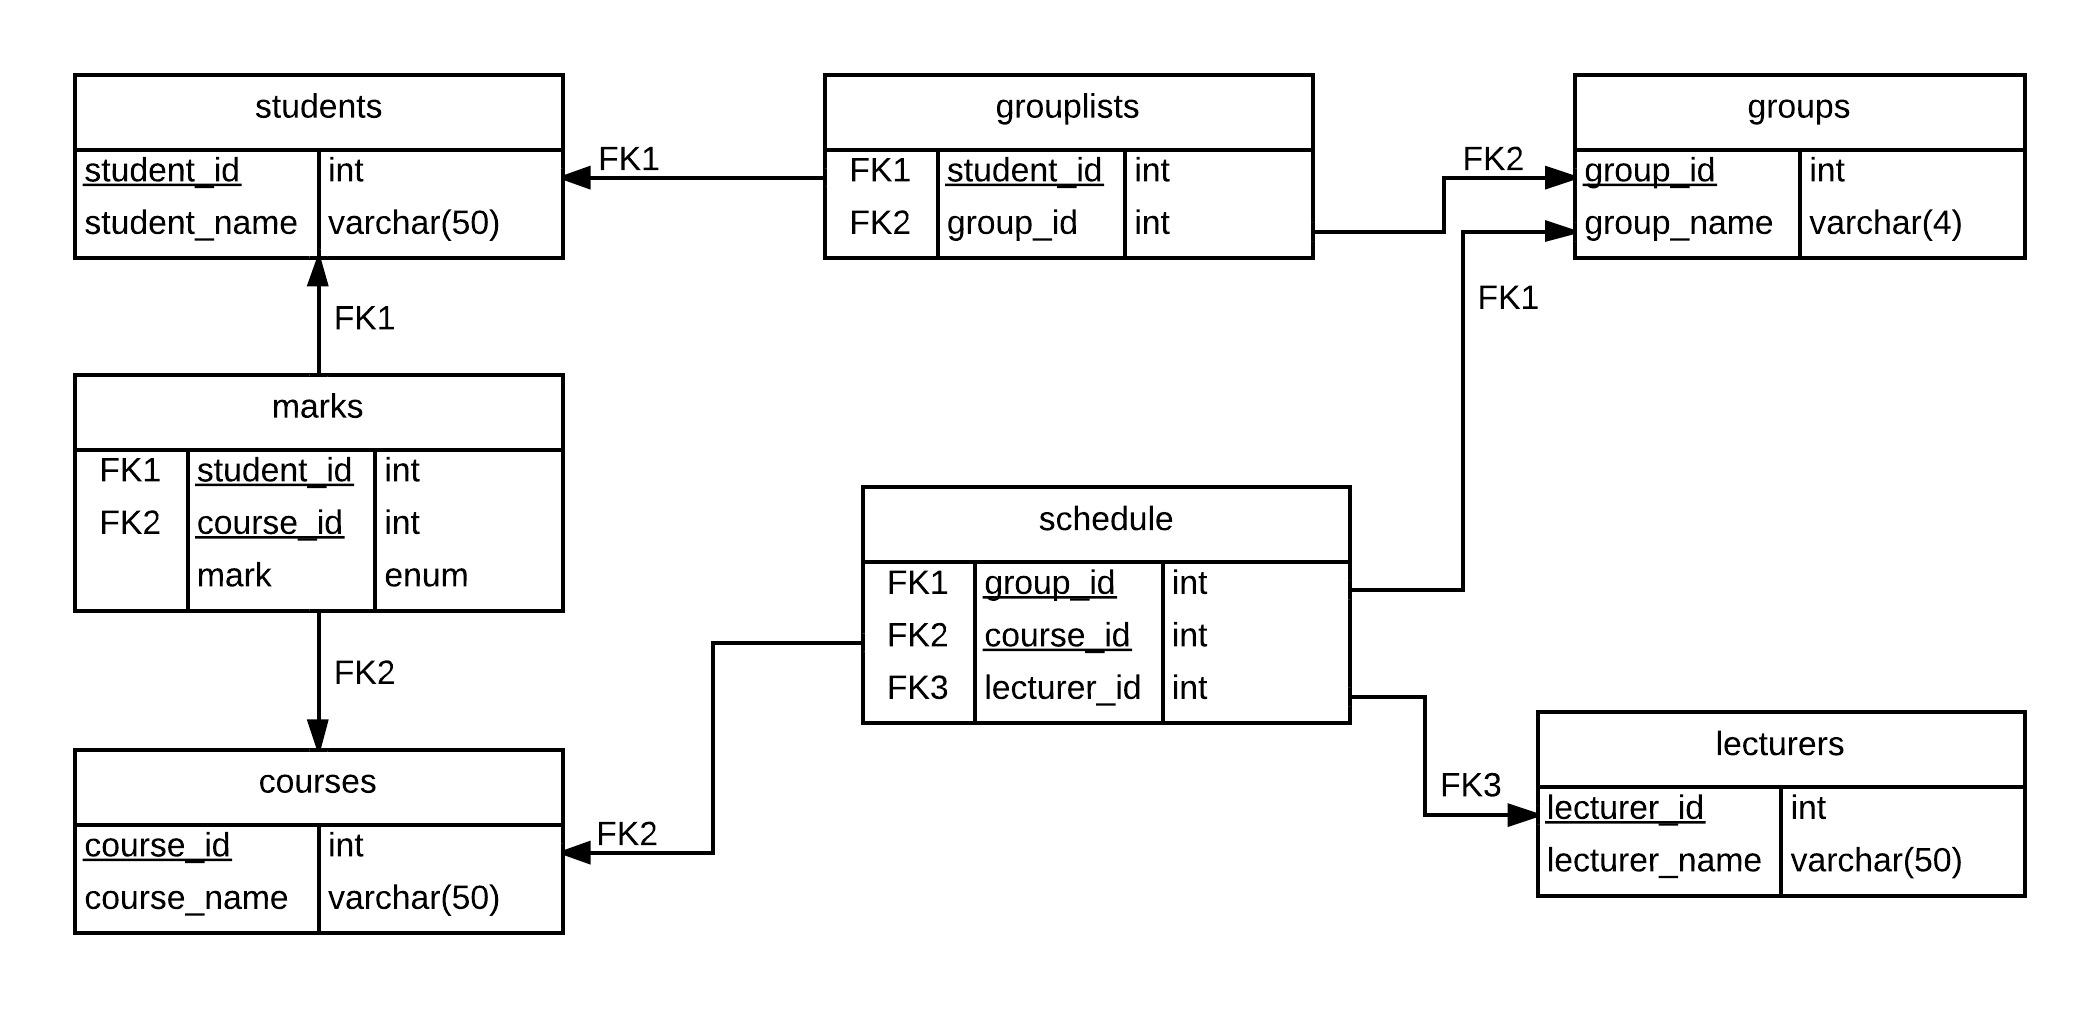
\includegraphics[scale=0.2]{pdm}
\end{center}

\begin{enumerate}

	\item {Информация о студентах с заданной оценкой по предмету «Базы данных».\\
	Пусть $X$ -- заданная оценка, тогда:\\
	$\pi_{student\_id, student\_name}(\sigma_{mark = X \wedge course\_name = 'Базы \: данных'}(marks \bowtie students \bowtie courses))$
	}


	\item {Информация о студентах не имеющих оценки по предмету «Базы данных».
		\begin{itemize}

			\item {среди всех студентов\\
			$students - \pi_{student\_id, student\_name}(\sigma_{course\_name = 'Базы \: данных'}(marks \bowtie students \bowtie courses))$
			}

			\item {среди студентов, у которых есть этот предмет\\
			$\pi_{student\_id, student\_name}(\sigma_{course\_name = 'Базы \: данных'}(schedule \bowtie courses \bowtie grouplists \bowtie students)) -$\\
			$\pi_{student\_id, student\_name}(\sigma_{course\_name = 'Базы \: данных'}(marks \bowtie students \bowtie courses))$
			}

		\end{itemize}
	}

	\item {Информация о студентах, имеющих хотя бы одну оценку у заданного лектора.\\
	Пусть $X$ -- идентификатор заданного лектора, тогда:\\
	$\pi_{student\_id, student\_name}(\sigma_{lecturer\_id = X}(students \bowtie marks \bowtie grouplists \bowtie schedule))$
	}

	\item {Идентификаторы студентов, не имеющих ни одной оценки у заданного лектора.\\
	Пусть $X$ -- идентификатор заданного лектора, тогда:\\
	$\pi_{student\_id}(students) - \pi_{student\_id}(\sigma_{lecturer\_id = X}(marks \bowtie grouplists \bowtie schedule))$
	}

	\item {Всех студентов, имеющих оценки по всем предметам заданного лектора.\\
	Пусть $X$ -- идентификатор заданного лектора, тогда:\\
	$\pi_{student\_name, course\_id}(\sigma_{lecturer\_id = X}(schedule \bowtie marks \bowtie students)) \div \pi_{course\_id}(\sigma_{lecturer\_id = X}(schedule))$
	}

	\item {Для каждого студента имя и курсы, которые он должен посещать.\\
	$\pi_{student\_name, course\_name}(students \bowtie grouplists \bowtie schedule \bowtie courses)$
	}

	\item {По лектору всех студентов, у которых он хоть что-нибудь преподавал.\\
	Пусть $X$ -- идентификатор заданного лектора, тогда:\\
	$\pi_{student\_name}(\sigma_{lecturer\_id = X}(schedule \bowtie grouplists \bowtie students))$
	}

\end{enumerate}

\end{document}